\chapter{Proposed Method}
%TODO: START COPY-PASTE
\section{Overview}
   %input output only melodic constrins
   %flow chart
      \begin{figure*}[tp]
         \begin{center}
            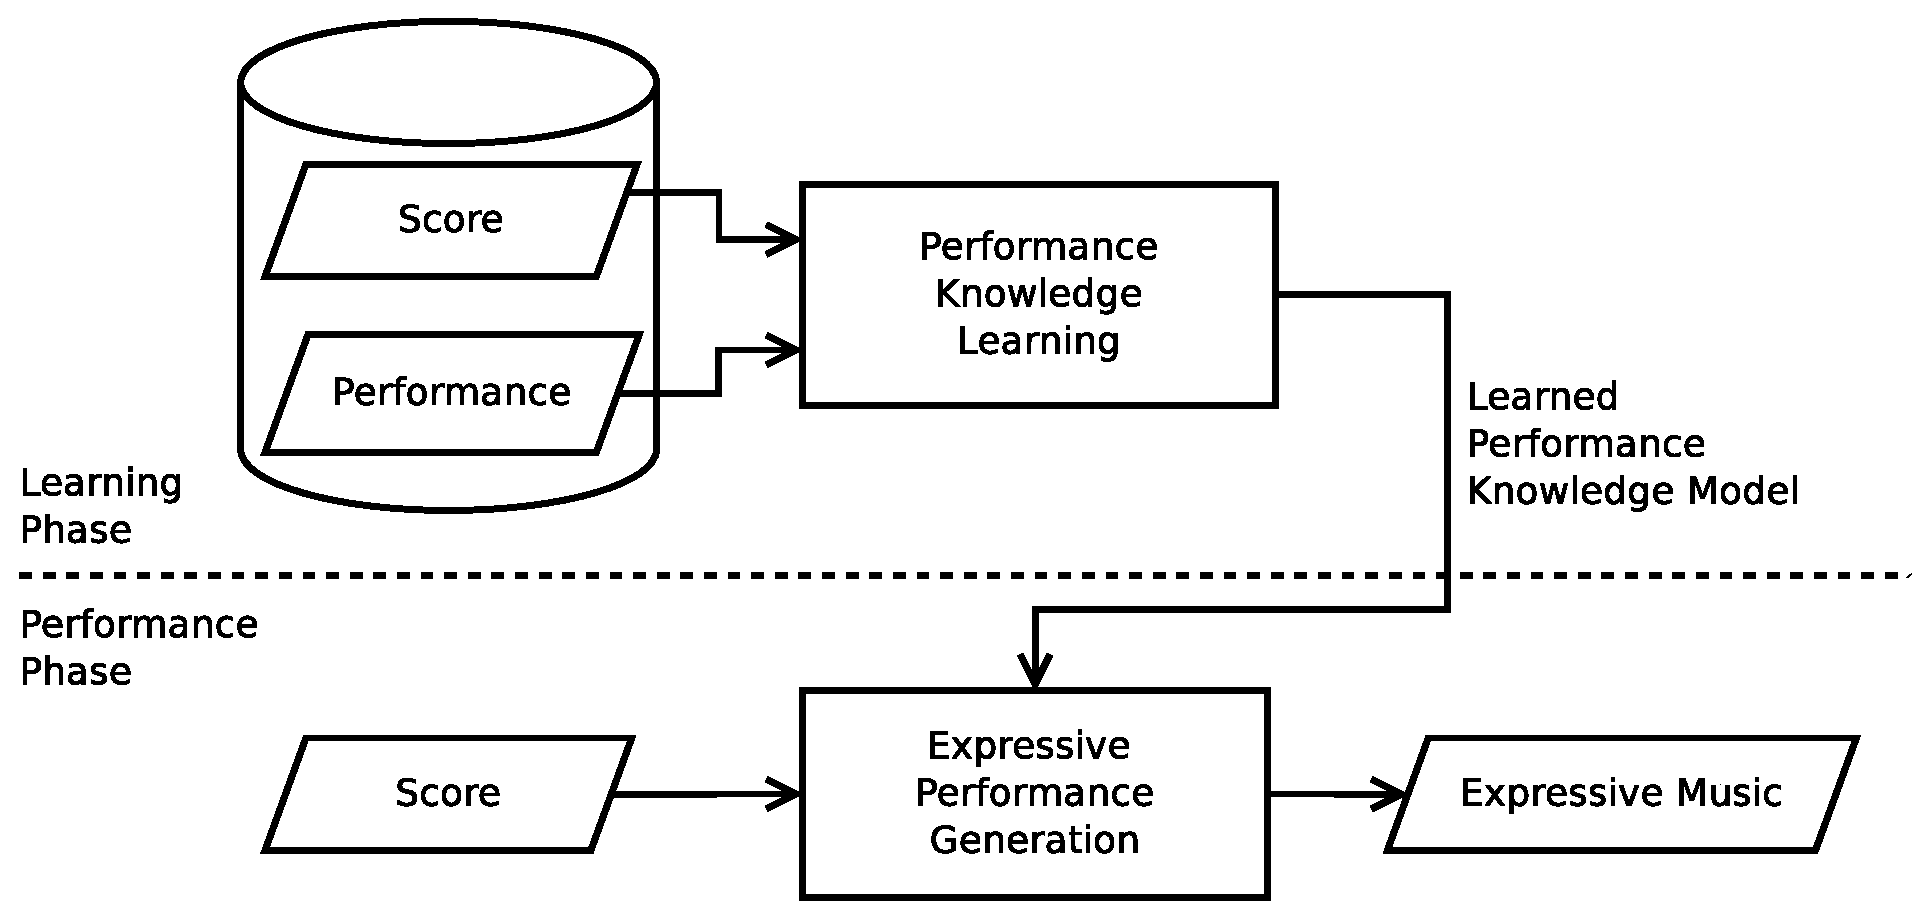
\includegraphics[width=\textwidth]{fig/high_lev_arch}
         \end{center}
         \caption{High Level System Architecture} 
         \label{fig:flow}
      \end{figure*}
The high-level architecture of the purposed system is shown in figure \ref{fig:flow}. The system has two phases, the upper half of the figure is the learning phase, while the lower half is the performing phase.  In the training phase, score and expressive performance recording pairs are feed in, they will serve as training examples for the machine learning algorithm, namely structural support vector machine with hidden markov model output (a.k.a SVM-HMM). The learning algorithm will produce a performance knowledge model, which can be used to generate expressive performance hereafter. In the performing phase, a score will be given to the system for expressive performance. The SVM-HMM generation module will use the performance knowledge learned in the previous phase to produce expressive performance. The SVM-HMM output then go through a MIDI generator and MIDI synthsizer to produce audible performance.
%TODO: refer to feature exction and corpus chapter

The system is not intend to add fixed expression to all pieces. Rather it is intended to perform music according to the style which the user wants. This kind of user interactivity can be achieved in two ways: first, the user can choose the training corpus. A user can select a subset of training sample to produce unique models. For example, if the corpus contains only one performer's recordings, the learned model will very likely have a unique style of the performer. Second, the phrasing of a song is given by the user. Since phrasing controls the overall structural interpretation of a music piece, and form a breathing feeling in music, user is given direct control over the performance.

There are still some constrains for the system now. The scores must be monophonic and contains only one musical phrase. One has to manually label the phrasing for any scores used. The learning algorithm, namely SVM-HMM, can only perform offline learning, so the learning phase can only work in a non-realtime scenario. The generating phase can work much faster though, it can produce expressive music almost instantaneously after loading the score. All the scores are loaded in batch, the system currently don't accept streaming input.

In the following sections, we will discuss the detail steps in the learning and performing phases, and some implementation detail used in each step. Since SVM-HMM learning requires features to be extracted from samples, we will discuss the features used in the end of this chapter.

%\chapter{Theoretical Background}
%\framebox{REVIEW1}
\section{A Brief Introduction to SVM-HMM}
\label{sec:svm-hmm}
In this thesis, we use structural support vector machine to learn performance knowledge from expressive performance samples. Unlike traditional SVM algorithm, which can only produce univariate prediction, structural SVM can produce structural predictions like tree, graph or sequence. Structural SVM with hidden Markov model output (SVM-HMM) has been successfully applied to part-of-speech tagging problem\cite{svm2009}. The part-of-speech tagging problem has some similarity with expressive performance problem. In part-of-speech tagging, one tries to identify the role by which the word plays in the sentence, while in expressive performance, one tries to determine how a note should be played, usually based on it's role in the musical phrase. %For example, an authentic cadence at the end of a phrase is usually played louder and stronger than a embellishment note in the middle of a phrase. 
Thus, we believe SVM-HMM will be a good candidate for expressive performance. The following introduction and formulas relies heavily on \cite{svm2009, svm2005, svm2003}.

%Ref: 20130420 slides

%TODO:discuss traditional SVM here?
Traditional SVM prediction problem can be described as finding a function 
$$h: \mathcal{X \rightarrow Y}$$ with lowest prediction error. $\mathcal{X}$ is the input features space, and $\mathcal{Y}$ is the prediction space. In traditional SVM, elements in $\mathcal{Y}$ are labels (classification) or real values (regression). But structural SVM extends the framework to generate structural output, such as tree, graph or sequence.
To extend SVM to support structured output, the problem is modified as finding a discriminant function $$F: \mathcal{X} \times \mathcal{Y} \rightarrow \mathcal{R}$$, in which the input/output pairs are mapped to a real number score. To predict an output $y$ for an input $x$, one try to maximize $F$ over all $y \in \mathcal{Y}$. 

$$f(x) = \argmax_{y\in\mathcal{Y}} F(w,x,y)$$

Let $F$ be a linear function of the form:

$$ F = \mathbf{w}^{T}\Psi(x,y)$$, 
where $\mathbf{w}$ is the parameter vector, and $\Psi(x,y)$ is the kernel function relating input $x$ to output $y$. $\Psi$ can be defined to accommodate various kind of structures. 

%emprical risk
For each structure we want to predict, a loss function that measures the accuracy of of a prediction is required. A loss function $\Delta:\mathcal{Y}\times\mathcal{Y}\rightarrow R$ need to satisfy the following property:

$$\Delta(y, y') \geq 0 \ for\ y \neq y'$$
$$\Delta(y, y) = 0 $$

The loss function is assumed to be bounded. Let's assume the input-output pair $(x,y)$ is drawn from a join distribution P(x,y), the prediction problem is to minimize the total loss:

%TODO: total loss formula 2005 sec 2.1
$$R_p^\Delta = \int_{\mathcal{X} \times \mathcal{Y}} \Delta (y, f(x))dP(x,y)$$

Since we can't directly find the distribution $P$, we need to replace this total loss with a empirical loss, which can be calculated from the observed training set of $(x_i, y_i)$ pairs.
%TODO: emprical loss
$$R_s^\Delta(f) = \frac{1}{n}\sum^n_{i=1}\Delta(y_i, f(x_i))$$

Now we are ready to extend SVM to structural output, starting with a linear separable case, and we will then extend it to soft-margin formulation. 

A linear separable case can be expressed by a set of linear constrains
%TODO: 2005 formula 4
$$\forall i \in \{1,\cdots,n\}, \forall \hat{y_i}\in\mathcal{Y}: \mathbf{w}^T [\Psi(x_i, y_i) - \Psi(x_i, \hat{y_i})]\geq 0$$

The constrains imply that the groundtruth $y_i$ for $x_i$ has the minimum $F$ value than any other $\hat{y}_i \neq {y_i}$.

The key concept of SVM is the large margin principle. We not only want to find a solution that statisfies the constrains, but also we want to maximize the margin between the groundtruth and the second best $\hat{y}_i$:
%TODO: 2005 formula 4+
$$
\begin{aligned}
& \max_{\gamma, \mathbf{w}:\|\mathbf{w}\| = 1} \gamma \\
& s.t \; \forall i \in \{1,\cdots,n\}, \forall \hat{y_i} \in\mathcal{Y}: \mathbf{w}^T [\Psi(x_i, y_i) - \Psi(x_i, \hat{y_i})] \geq \gamma\\
\end{aligned}
$$

, which is equivalent to the convex quadratic programming problem:
%TODO: 2005 formula 5,k 6
$$
\begin{aligned}
   & \min_{\mathbf{w}, \xi_i \geq 0} \frac{1}{2}\|\mathbf{w}\|^2 \\\
    &s.t.\; \forall i \in \{1,\cdots,n\},\hat{y_i} \in \mathcal{Y}: \mathbf{w}^T[\Psi(x_i,y_i) - \Psi(x_i,\hat{y_i})] \geq 1\\
\end{aligned}
$$

To extend the linear-separable case to non-separable case, slack variables $\xi_i$ can be introduced to penalize prediction errors, results in a soft-margin formalization:
%TODO: 2005 formula SVM1
$$
\begin{aligned}
   & \min_{\mathbf{w}, \xi_i \geq 0} \frac{1}{2}\|\mathbf{w}\|^2 + \frac{C}{n}\sum^n_{i=1}\xi_i\\
    &s.t.\; \forall i \in \{1,\cdots,n\},\hat{y_i} \in \mathcal{Y}: \mathbf{w}^T[\Psi(x_i,y_i) - \Psi(x_i,\hat{y_i})] \geq 1 - \xi_i \\
\end{aligned}
$$

$C$ is the weighting parameter controlling the trade-off between low training error and large margin. The optimal $C$ varies between different problems, so experiment should be conducted to find the optimal $C$ for our problem.

Intuitively, a constrain violation with larger loss should be penalize more than the one with smaller loss. So I. Tsochantaridis et al. \cite{svm2005} proposed two possible way to take the loss function into account. The first way is to re-scale the slack variable by the inverse of the loss, so a high loss leads to smaller re-scaled slack variable:
%slack rescaling

$$
\begin{aligned}
   & \min_{\mathbf{w}, \xi_i \geq 0} \frac{1}{2}\|\mathbf{w}\|^2 + \frac{C}{n} \sum^n_{i=1}\xi_i\\
    &s.t.\; \forall i \in \{1,\cdots,n\},\hat{y_i} \in \mathcal{Y}: \mathbf{w}^T[\Psi(x_i,y_i) - \Psi(x_i,\hat{y_i})] \geq 1 - \frac{\xi_i}{\Delta(y_i, \hat{y_i})} \\
\end{aligned}
$$

The second way is to re-scale the margin, which yields 
%margin-rescaling
$$
\begin{aligned}
   & \min_{\mathbf{w}, \xi_i \geq 0} \frac{1}{2}\|\mathbf{w}\|^2  + \frac{C}{n} \sum^n_{i=1}\xi_i\\
    &s.t.\; \forall i \in \{1,\cdots,n\},\hat{y_i} \in \mathcal{Y}: \mathbf{w}^T[\Psi(x_i,y_i) - \Psi(x_i,\hat{y_i})] \geq \Delta(y_i, \hat{y_i}) - \xi_i\\
%
\end{aligned}
$$
In the implementaion we use, we use margin re-scaling.

But the above quadratic programming problem has a very large number ($O(n|\mathcal{Y}|)$) of constrains, which will take considerable time to solve. I. Tsochantaridis et al. \cite{svm2005} proposed a greedy algorithm to speed up the process by selecting only part of the constrains that contributes the most to finding the solution. Initially, the solver starts with an empty working set containing no constrains. Than the solver iteratively scans the training set to find the most violated constrains under the current solution. If a constrain is violated more times than a desired threshold, the constrain is added to the working set of constrains. Then the solver re-calculate the solution under the new working set. The algorithm will terminate once no more constrain can be added under the desired precision.

In a later work by Joachims et al.\cite{svm2009}, they created a new formulation and algorithm to further speed up the algorithm. Instead of using one slack variables for each training sample, which results in a total of $n$ slack variables, they use a single slack variable for all $n$ training samples. The following formula is the 1-slack version of slack-rescaling structural SVM:
%1-slack
$$
\begin{aligned}
    & \min_{\mathbf{w}, \xi_i \geq 0} \frac{1}{2}\|\mathbf{w}\|^2  + C \xi\\
    &s.t.\; \forall i \in \{1,\cdots,n\},\hat{y_i} \in \mathcal{Y}: \mathbf{w}^T[\Psi(x_i,y_i) - \Psi(x_i,\hat{y_i})] \geq \frac{1}{n}\sum^n_{i=1}1 - \frac{\xi}{\Delta(y_i, \hat{y_i})} \\
\end{aligned}
$$

And margin-rescaling structural SVM:

$$
\begin{aligned}
    & \min_{\mathbf{w}, \xi_i \geq 0} \frac{1}{2}\|\mathbf{w}\|^2  + C \xi\\
    & s.t.\; \forall i \in \{1,\cdots,n\},\hat{y_i} \in \mathcal{Y}: \mathbf{w}^T[\Psi(x_i,y_i) - \Psi(x_i,\hat{y_i})] \geq \frac{1}{n}\sum^n_{i=1}\Delta(y_i, \hat{y_i}) - \xi \\
\end{aligned}
$$
%                $$\min_{\mathbf{w}, \xi_i \geq 0} \frac{1}{2}\mathbf{w}^T\mathbf{w} + \frac{C}{n} \sum_{i=1}^{n} \xi_i$$
%                s.t. for $i = 1\cdots n$
%                $$\forall \hat{y_i} \in \mathcal{Y}: \mathbf{w}^T[\Psi(x_i,y_i) - \Psi(x_i,\hat{y_i})] \geq \Delta(y_i, \hat{y_i}) - \xi_i $$
%
%                $$\forall \hat{y_i} \in \mathcal{Y}: \mathbf{w}^T[\Psi(x_i,y_i) - \Psi(x_i,\hat{y_i})] \geq 1 - \frac{\xi+i}{\Delta(y_i, \hat{y_i})}$$
Detailed proof on how the new formulation is equally general as the old one is given in the paper \cite{svm2009}.

With the framework described above, the only problem left is how to define the general loss function and $\Psi$ for our problem? Drawing the inter-state dependencies and time dependencies concept from hidden Markov model, Y. Altun et al.\cite{svm2003} proposed two types of features for a equal-length observation/label sequence pair $(x,y)$. The first is the interaction of a observed feature $x^s$ with a label $y^t$, the other is the interaction between neighboring labels $y^s$ and $y^t$. 

%   \begin{figure*}[tp]
%      \begin{center}
%         \includegrapsics[width=0.8\textwidth]{fig/TBDFigure}
%      \end{center}
%      \caption{Hidden Markov Model}
%      \label{fig:hmm}
%   \end{figure*}

To illustrate the method, we use a example from music: for some observed features $\Psi_r(x^s)$ of a note $x$ located in $s$-th position of the phrase, and assume $\left[ \left[ y^t = \tau \right] \right]$ denotes the $t$-th note is played at a velocity of $\tau$, the interaction of the observed feature and the label can be written as:
%TODO hmm 3 formula 4
$$\psi^{st}_{r\sigma}(\mathbf{x}, \mathbf{y}) = \left[\left[y^t = \tau \right] \right]\Psi_r(x^s),\; 1\leq\gamma\leq d,\; \tau \in \Sigma $$

And the interaction between labels can be written as:
%TODO hmm 3 formula 5
$$\hat{\psi}^{st}_{r\sigma}(\mathbf{x}, \mathbf{y}) = \left[\left[y^s = \sigma \wedge y^t = \tau \right] \right],\; \sigma, \tau \in \Sigma $$

By selecting a order of dependency for the HMM model, we can further restrict $s$'s and $t$'s. For example, for a first-order HMM, $s = t$ for the first feature, and $s = t-1$ for the second feature. The two features on the same time $t$ is then stacked into a vector $\Psi(x,y;t)$. The feature map for the whole sequence is simply the sum of all the feature vectors 

%TODO hmm 3 formula 6
$$\Psi(\mathbf{x}, \mathbf{y}) = \sum^T_{t=1}\Psi(\mathbf{x}, \mathbf{y};t)$$

The distance, i.e. the general loss function, between two feature maps depends on the number of common label segments and the inner product between the input features sequence with common labels.


$$\Delta(\Psi(\mathbf{x}, \mathbf{y}), \Psi(\mathbf{\hat{x}}, \mathbf{\hat{y}})) = \sum_{s,t}\left[\left[y^{s-1} = \hat{y}^{t-1}\wedge y^s = \hat{y}^t\right] \right] + \sum_{s,t}\left[\left[y^{s} = \hat{y}^{t}\right] \right]k(x^s, \hat{x}^t)$$

Finally, during the prediction process, a Viterbi-like decoding algorithm is used to effeciently find a $y$ that maximize $F$.


%TODO: how to define loss function for HMM?
%(2003) section 3
%ovserved output <--> tag
%previous tag <--> this tag (1-order markov)
% Psi = each note's above two property summed up
%similarity = same prev tag <--> this tag sequence + same tag <--> observed output distance

%Hard-margin one
%Soft-margin one => introduce slack variable 
%Example with large loss should be emphasized => slack rescaling
%Margin can also be scaled => margin rescaling
%There are too many constrains => greedy algo (2005), select a subset of constrains from the most violated constrains to solve
%To speed up, n-slack variables are reduced to 1-slack variable (2009)

%           \item Prediction error (risk):
%               $$R^\Delta_p(h) = \int_{\mathcal{X}\times\mathcal{Y}}\Delta(y, h(x)) dP(x,y)$$
%               \begin{tabular}{ll}
%                   where & $\Delta()$ is the loss function \footnote{Must satisfy $\Delta(x,x) = 0$, $\Delta(x,y) > 0$}\\
%                   & P(x,y) is the joint distribution of $\mathcal{X}$ and $\mathcal{Y}$
%               \end{tabular}

%    \begin{frame}{Emperical Risk}
%       \begin{itemize}
%           \item Emperical Risk from training sample $S$:\footnote{Emperical Risk Minimization Priciple (Vapnik V (1998) Statistical Learning Theory. Wiley, Chichester, GB)}

%               $$R^\Delta_S(h) = \frac{1}{n}\sum_{i=1}^{n}\Delta(y_i, h(x_i))$$
%                   where  $\Delta()$ is the loss function 

%           \item Classification SVM

%                   $$\displaystyle \min_{\mathbf{w}, \xi_i \geq 0} \frac{1}{2}\mathbf{w}^T\mathbf{w} + \frac{C}{n} \sum_{i=1}^{n} \xi_i$$
%                   s.t. $$\forall i\in {1,\cdots n}: y_i (\mathbf{w}^T x_i) \geq 1-\xi_i$$
                  

%           \item Learn a discriminant function $f:\mathcal{X} \times \mathcal{Y} \rightarrow \Re$ 
%           \item Given $x$, maximizing $f$ over all $y \in \mathcal{Y}$
%               $$h_\mathbf{w} (x) = \argmax_{y\in\mathcal{Y}} f_\mathbf{w} (x,y)$$
%           \item 
%               in which $$f_\mathbf{w} (x,y) = \mathbf{w}^T{\Psi}(x,y)$$
%               \begin{tabular}{ll}
%                   where & $\mathbf{w} \in \Re^N$ is a parameter vector\\
%                         & $\Psi(x,y)$ is a feature vector relating $x$ and $y$
%               \end{tabular}
              

 
% \section{Structural SVM}

% \section{Theoretical Details}
% %&=& &=& &=& &=& &=& &=& &=& &=& =
%    \begin{frame}{Lowest Risk}
%       \begin{itemize}
%           \item Prediction error (risk):
%               $$R^\Delta_p(h) = \int_{\mathcal{X}\times\mathcal{Y}}\Delta(y, h(x)) dP(x,y)$$
%               \begin{tabular}{ll}
%                   where & $\Delta()$ is the loss function \footnote{Must satisfy $\Delta(x,x) = 0$, $\Delta(x,y) > 0$}\\
%                   & P(x,y) is the joint distribution of $\mathcal{X}$ and $\mathcal{Y}$
%               \end{tabular}

%           %\item Training sample: $(x_1, y_1), (x_2, y_2), \cdots$ where $y_i$'s may have structural relationship
              
%       \end{itemize}
%    \end{frame}
%    \begin{frame}{Emperical Risk}
%       \begin{itemize}
%           \item Emperical Risk from training sample $S$:\footnote{Emperical Risk Minimization Priciple (Vapnik V (1998) Statistical Learning Theory. Wiley, Chichester, GB)}

%               $$R^\Delta_S(h) = \frac{1}{n}\sum_{i=1}^{n}\Delta(y_i, h(x_i))$$
%                   where  $\Delta()$ is the loss function 

%           %\item Training sample: $(x_1, y_1), (x_2, y_2), \cdots$ where $y_i$'s may have structural relationship
              
%       \end{itemize}
%    \end{frame}

%    \begin{frame}{Traditional SVM}
%       \begin{itemize}
%           \item Classification SVM

%                   $$\displaystyle \min_{\mathbf{w}, \xi_i \geq 0} \frac{1}{2}\mathbf{w}^T\mathbf{w} + \frac{C}{n} \sum_{i=1}^{n} \xi_i$$
%                   s.t. $$\forall i\in {1,\cdots n}: y_i (\mathbf{w}^T x_i) \geq 1-\xi_i$$
                  

              
%       \end{itemize}
%    \end{frame}

%    \begin{frame}{Structural SVM}
%       \begin{itemize}
%           \item Extend SVM for structural output
%           \item Learn a discriminant function $f:\mathcal{X} \times \mathcal{Y} \rightarrow \Re$ 
%           \item Given $x$, maximizing $f$ over all $y \in \mathcal{Y}$
%               $$h_\mathbf{w} (x) = \argmax_{y\in\mathcal{Y}} f_\mathbf{w} (x,y)$$
%           \item 
%               in which $$f_\mathbf{w} (x,y) = \mathbf{w}^T{\Psi}(x,y)$$
%               \begin{tabular}{ll}
%                   where & $\mathbf{w} \in \Re^N$ is a parameter vector\\
%                         & $\Psi(x,y)$ is a feature vector relating $x$ and $y$
%               \end{tabular}


                  

              
%       \end{itemize}
%    \end{frame}

%    \begin{frame}{N-slack Formulations}
%       \begin{itemize}
%           \item margin-rescaling: change hinge, fixing slope
%              $$\Delta_{MR}(y,h_\mathbf{w}) = \max_{\hat{y} \in \mathcal{Y}} \{ \Delta(y, \hat{y}) - \mathbf(x)^T {\Psi}(x,y) + \mathbf{w}^T{\Psi}(x,\hat{y}\} \geq \Delta(y,h_\mathbf{w}(x))$$
%           \item slack-rescaling: fixing hinge, changing slope
%              $$\Delta_{SR}(y,h_\mathbf{w}) = \max_{\hat{y} \in \mathcal{Y}} \{ \Delta(y, \hat{y}) (1 - \mathbf(x)^T {\Psi}(x,y) + \mathbf{w}^T{\Psi}(x,\hat{y} )\} \geq \Delta(y,h_\mathbf{w}(x))$$
              
%       \end{itemize}
%    \end{frame}

%    \begin{frame}{Optimization Problems}
%       \begin{itemize}
%           \item
%                $$\displaystyle \min_{\mathbf{w}, \xi_i \geq 0} \frac{1}{2}\mathbf{w}^T\mathbf{w} + \frac{C}{n} \sum_{i=1}^{n} \xi_i$$
%                s.t. for $i = 1\cdots n$
%           \item n-slack structural SVM w/ margin-rescaling
%                $$\forall \hat{y_i} \in \mathcal{Y}: \mathbf{w}^T[\Psi(x_i,y_i) - \Psi(x_i,\hat{y_i})] \geq \Delta(y_i, \hat{y_i}) - \xi_i $$

%           \item n-slack structural SVM w/ slack-rescaling
%                $$\forall \hat{y_i} \in \mathcal{Y}: \mathbf{w}^T[\Psi(x_i,y_i) - \Psi(x_i,\hat{y_i})] \geq 1 - \frac{\xi+i}{\Delta(y_i, \hat{y_i})}$$
%       \end{itemize}
%    \end{frame}

%    \begin{frame}{1-Slack Formulation}
%       \begin{itemize}
%           \item
%       \end{itemize}
%    \end{frame}


%TODO: theoratical background


%\section{Brent's Method}
%\section{diff}

\section{Learning Performance Knowledge}

\begin{figure*}[tp]
   \begin{center}
      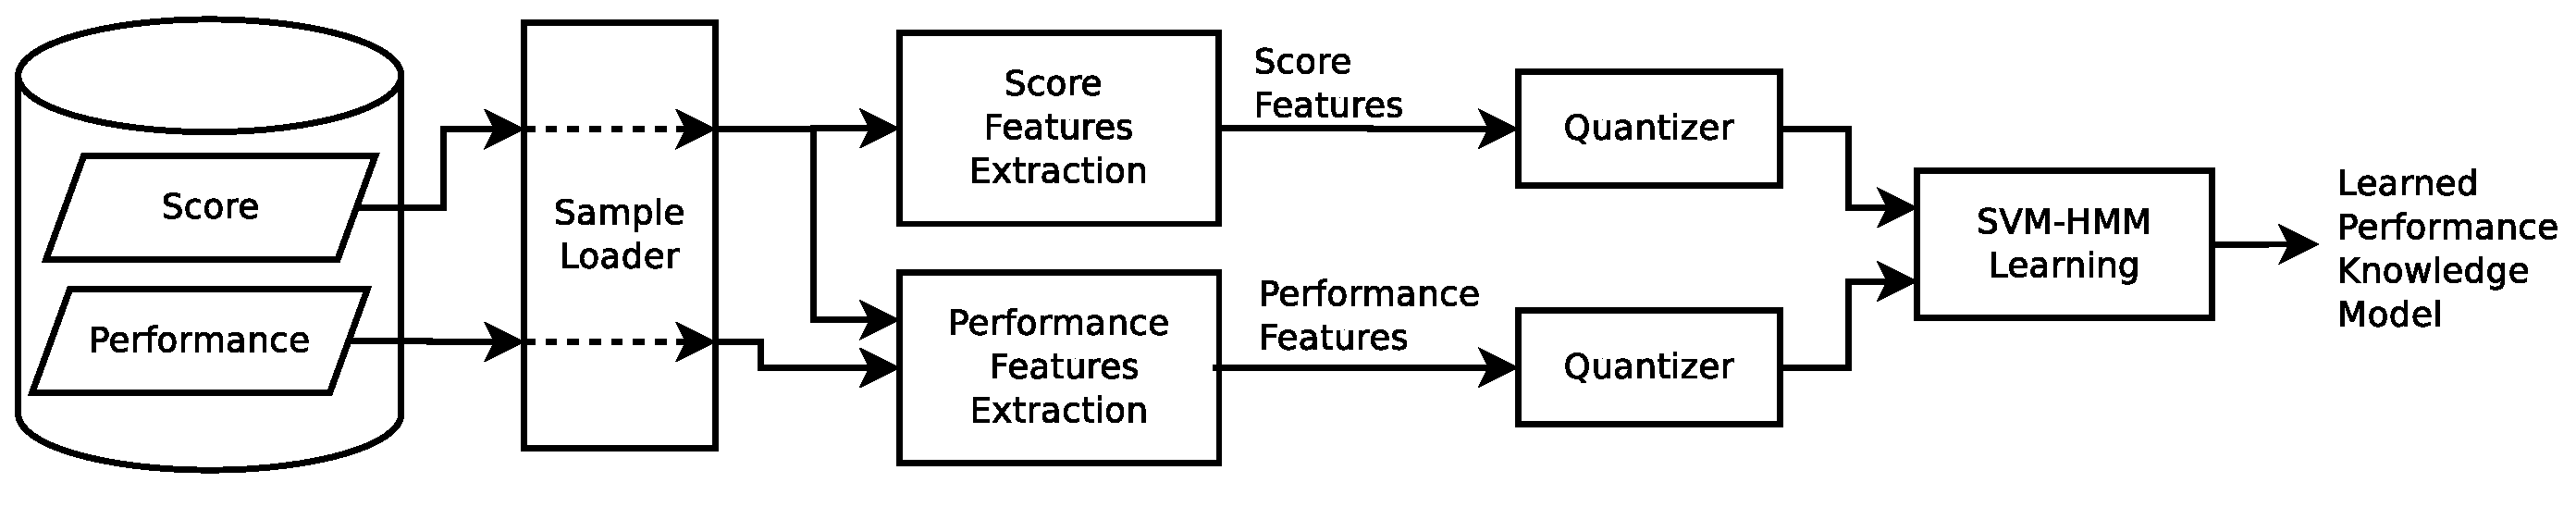
\includegraphics[width=\textwidth]{fig/learn_arch}
   \end{center}
   \caption{Learning Phase Flow Chart} 
   \label{fig:learnflow}
\end{figure*}
The main goal in the learning phase is to extract performance knowledge from training samples. Figure \ref{fig:learnflow} shows the internal structure of the learning phase.

   Training samples are matched score and expressive performance pairs (their format and preparation process is discussed in Chapter \ref{chap:corpus}). The training samples are loaded as machine-readable format, and have their features extracted. Two types of features will be extracted from the samples, first, the information from the score only are called score features; second, the information of the expressive performance with respect to the score is called the performance features. In order to generate new expressive performance, we want to learn a prediction model by which we can predict the performance features given the score model. This process can be analogize to a human performer reading the explicit and implicit cues from the score, and perform the music with certain expressive expression. The learning part is done by a supervised learning algorithm. In this thesis, we choose Structural Support Vector Machine with Hidden Markov Model Output (SVM-HMM) as our learning algorithm.


% The learning module has a input/output interface that is independent of the underlying algorithm, so different algorithm can be implemented without changing the overall structure of the system.

%TODO: sample loader
\subsection{Training Sample Loader}
   A training sample is loaded with the sample loader module, since a training sample is consisted of a score (musicXML format) and an expressive recording (MIDI format), the sample loader finds the two files given the sample name, and load them into an intermediate representation (\texttt{music21.Stream} object provided by the \texttt{music21} library\cite{music21} from MIT). The music21 library will convert the musicXML and MIDI format into a python Object hierarchy that is easy to access and manipulate by python code. The loaded score are then handed to the feature extractor module. 

One caveat here is that the recording in MIDI may contain very subtle expression. But the music21 library will quantize the MIDI in the time axis by default, which will destroy the subtle onset and duration expression. And the music21 library don't handle the "ticks per quarter note" information in the MIDI header\cite{midispec}, so we must explicitly specify that this value, and disable quantization during MIDI loading.

\subsection{Features Extraction}
   In  order to keep the system architecture simple, a feature extractor are designed to be independent to other feature extractors, so features can added or removed without affecting the rest of the system. And further more, this enables parallel processing during feature extraction. To achieve this, each feature must implement a common feature extractor interface, and feature extractors should not communicate with each other. 

   But sometimes a feature inevitably depends on other features, for example, the "relative duration with the previous note" is calculated based on the "duration" feature. But since we want to avoid complex scheduling with dependency, the "duration" feature is extracted during the extraction of the "relative duration" feature, no matter if the "duration" feature is extracted prior of after the "relative duration". Therefore, the "duration" feature extracted has computed twice. To avoid redundant computation of the feature extractors, we implemented a caching mechanism. Say, the "duration" feature had been computed once, it's value will be cached during this execution session; when the "relative duration" extractor calls the "duration" extractor again, the value is retrieved from cache without re-calculation. This method can speed up the execution while keeping the system complexity low.

   The extracted features are aggregated and stored into a JavaScript Object Notation (JSON) file. By saving the features in a human-readable intermediate file, the researcher can easily look into the file to debug potential problems.%the learning module can then load this file as inpu.t. The learning algorithm can then do any pre-processing on the features, such as aggregation or quantization. The output of this module is the algorithm specific model description. For example, a linear regression algorithm will output the regression parameters. The algorithm is required to produce a model file containing the model description, but the system doesn't care about the internal format of the model description file, it will simply feed this model file to the generation module in the generation stage. So the developer of the learning module has to implement methods to write and read the model file themselves.

   %In the early stage of this research, linear regression is used. The results of linear regression is shown in \cite{Lyu2012}. In this thesis, Structural Support Vector Machine\cite{Joachims2009} is used instead. The detail of Structural SVM will be in the next Chapter.

\subsection{SVM-HMM Learning}
After all features are extracted, the next step is to learn performance knowledge from the features. In the early stage of this research, we have tried linear regression with limited success\cite{Lyu2012}. However, the assumption of linearity is an oversimplification. So we switch to Structural Support Vector Machine with Hidden Markov Model Output (SVM-HMM)\cite{svm2009, svm2005, svm2003}  as our supervised learning algorithm. 

The SVM-HMM learning module loads the JSON file from the previous stage, and rearrange the features to fit the required input format of the SVM-HMM learner program. However, the features from the previous stage are real numbers, but SVM-HMM only takes discrete output, so quantization is required here. For each feature, the quantizer calculates the overall mean and standard deviation from all training samples. Then the quantizer divides the range between mean minus three standard deviations to mean plus three standard deviations into 1024 intervals. Feature values below mean minus three standard deviations are quantized to the lowest bin, while values larger than mean plus three standard deviations are quantized to the highest bin. The range of three standard deviation and 1024 intervals are chosen by experience, which can be modified to fit different corpus.

The theoretical background of SVM-HMM is already described in Section \ref{sec:svm-hmm}, to implement the algorithm we leverage Thorsten Joachims's implementation called $SVM^{hmm}$ \cite{Joachims2008}. $SVM^{hmm}$ is an implementation of structural SVMs for sequence tagging \cite{svm2003} using the training algorithm described in \cite{svm2005} and \cite{svm2009}. The $SVM^{hmm}$ package contains a model training program called \texttt{svm\_hmm\_learn} and a model prediction program called \texttt{svm\_hmm\_classify}, which will be used in the performing phase. For structural simplicity, we train a separate model for each quantized performance feature, each model uses all the quantized score features to try to predict a single performance model. The\texttt{svm\_hmm\_learn} takes a training file describing those features. Each line represents features for a note, organized in the following format:
\begin{lstlisting}
	PERF qid:EXNUM FEAT1:FEAT1_VAL FEAT2:FEAT2_VAL ... #comment
\end{lstlisting}
\texttt{PERF} is a quantized performance feature. The \texttt{EXNUM} after \texttt{qid:} identifies the phrases, all notes in a phrase will have the same \texttt{qid:EXNUM} identifier. Following the identifier are quantized score features, denote as \texttt{feature name : feature value}, separated by space. And anything after the \texttt{\#} is comments.  An example of the training file is shown in Figure \ref{fig:expinput}

\begin{figure*}[tp]
   \begin{center}
      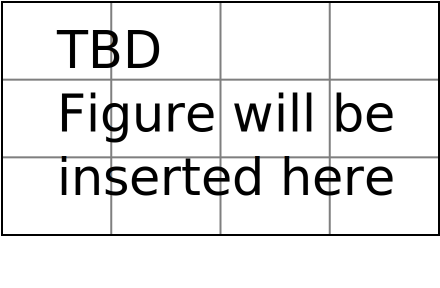
\includegraphics[width=\textwidth]{fig/TBDFigure}
   \end{center}
   \caption{Example input file} 
   \label{fig:expinput}
\end{figure*}

There are some key parameters need to be specified for the training process. First the $C$ parameter in SVM, which controls the trade-off between low training error and large margin. Larger C will result in lower training error, but the margin may be smaller. Second, the $\epsilon$ parameter controls the required precision for the constrains. The smaller the $\epsilon$, the precision will be higher, but may require more computation. Finally, for the HMM part, we need to specify the order of dependencies of transition states and emission states. In our case, transition dependency is set to one, which stands for first-order Markov property, and emission dependency is set to zero. Since we train separate models for each performance feature, each model can have their own set of parameters. The parameter selection process is done by experiment, which will be presented in Chapter \ref{chap:exp}

Finally, the training program will output three model files (because we use three performance features). In the model file are binary representation of the SVM-HMM model parameters, such as the support vectors and other informations, which represents the performance knowledge learned.  Since it takes considerable time to train a model (depending on the amount of training samples and the power of the computer running the system), the system can only support offline learning. But the learning process only need to be run once. The performance knowledge model can be reused over and over again in the performing phase.



\framebox{BOOKMARK}
   \section{Expressive Performance}
\begin{figure*}[tp]
   \begin{center}
      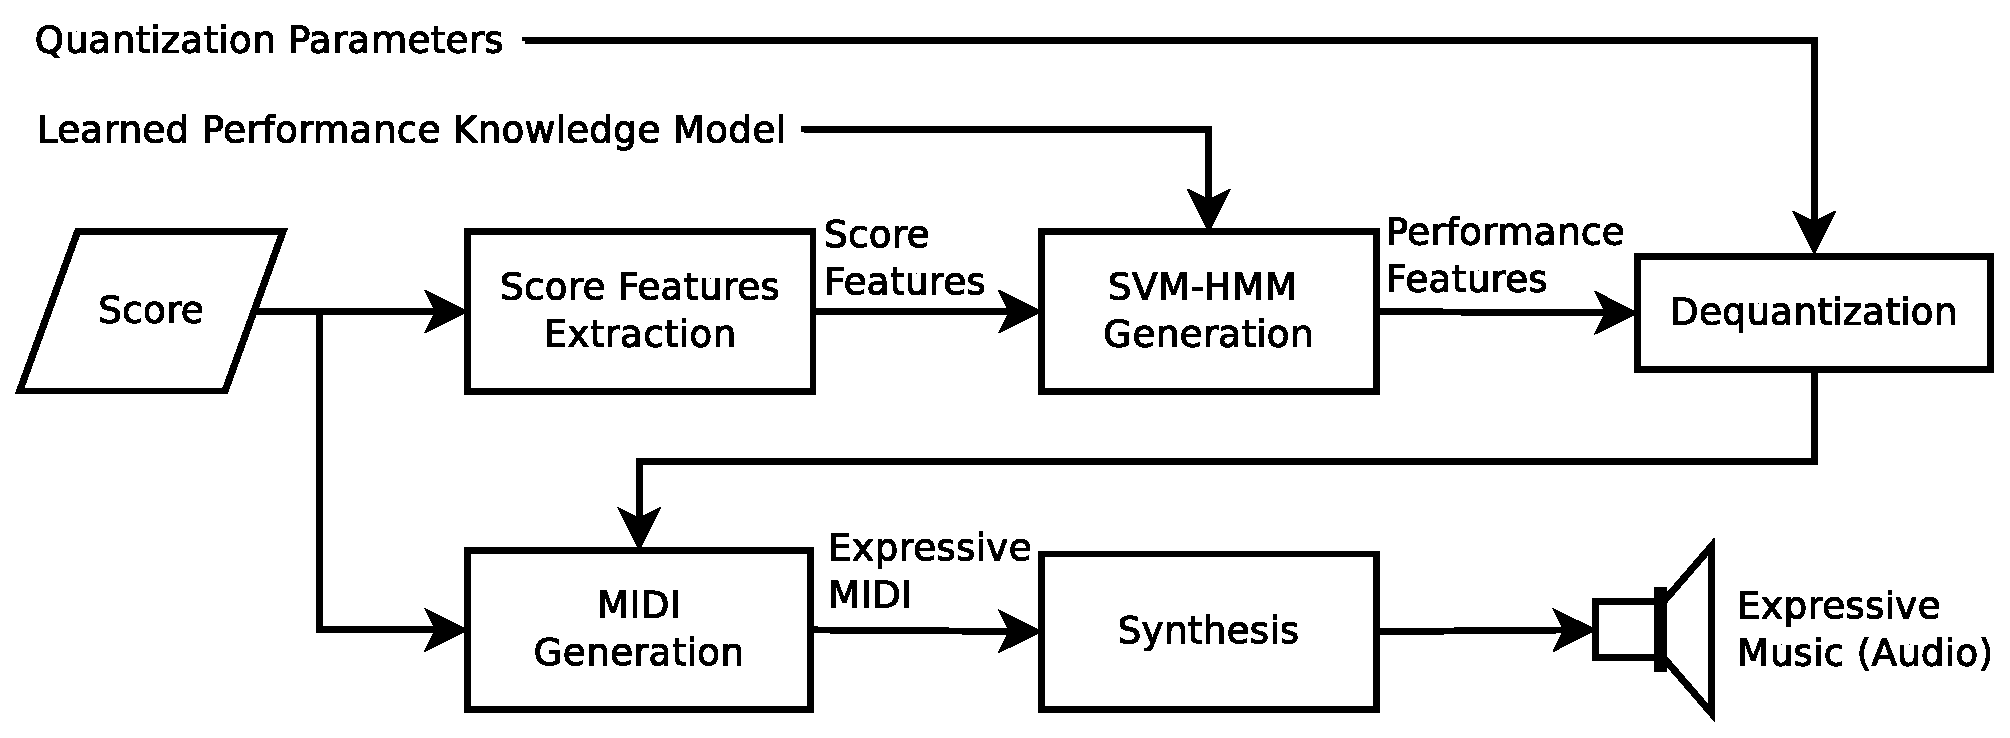
\includegraphics[width=\textwidth]{fig/perf_arch}
   \end{center}
   \caption{Performing Phase Flow Chart} 
   \label{fig:perfflow}
\end{figure*}
   \subsection{Feature Extraction and SVM-HMM Generation}
      After the model for a input phrase is generated, we can than use the score features and model coefficients to calculated the performance parameters. These performance parameters will then be applied to the input score.
      
      %TODO: no post-processing now
      %TODO: scaleable post-processing?
      Some post-processing will be made for each performance parameters: The first time bias will be reduced if it is too negative and create a negative onset time for the first note. Loudness will be shift and shrink to a predefined range. The default is 80~127 MIDI loudness level. This will ensure the loudness in the output will be in acceptable range. 
      
      \subsection{MIDI Generation}
      \framebox{TODO:Expend this generation}
 So after we input an input score, its score features will be extracted. These score features combined with regression model will be used to calculate performance features. The result will be an expressive MIDI output. Ready to be played by hardware or software synthesizer.  
 \framebox{TODO:off-line vs on-line}
 \framebox{TODO:Discuss timber and instrument specific techniques}
 \framebox{TODO:Discuss timber and instrument specific techniques}
   
%TODO:END COPY-PASTE
   \section{Features}
   The system is trying to mimic the process of human performance: the musican reads the explict and implict cues from the score and transform them into musical expressions. So the features can be categorized into two category: score features and performance features.  Score features are information contained in the score. Performance features corresponds to the musical expression. The basic time unit for both features are a note. 
      \subsection{Score Features}
      Score features includes:
      \begin{description}
         \item [Relative position in a phrase:]
            The relative position of a note in the phrase. From 0\% to 100\%. This feature can catch the musical hint of the opening and closing of a phrase.  
         \item [Relative pitch:]
            The pitch (in semitone) of a note relative to the pitch range of the phrase. For a phrase of $n$ notes with pitch $P_1, P_2, \dots, P_n$, $$RP = \frac{P_i -min(P_1, P_2, \dots, P_n) }{max(P_1, P_2, \dots, P_n)-min(P_1, P_2, \dots, P_n) }$$  Where $P_i$ is the pitch of note at position $t$

         \item [Interval from the previous note:] The direction of melody movement. Measured in semitone. $$IP = P_{i} - P_{i-1} $$ See figure \ref{fig:interval} for example.
         \item [Interval to the next note:] The direction of melody movement. $$IN = P_{i+1} - P_i$$ See figure \ref{fig:interval} for example.
         
      \begin{figure}[tp]
         \begin{center}
            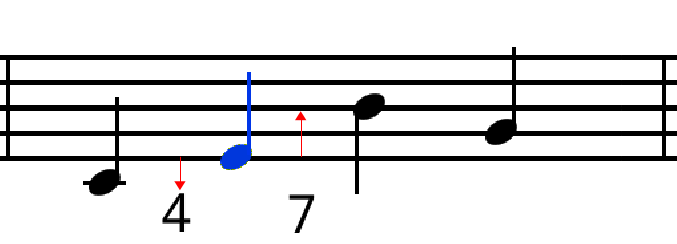
\includegraphics[width=0.4\textwidth]{fig/interval_arrow}
         \end{center}
         \caption{Interval from/to neighbor notes}
         \label{fig:interval}
      \end{figure}

         
         \item [Note duration:] The duration of a note in beats.
            \framebox{TODO: discuss how grace notes are handled, currently its duration is set to 0.0625 quarter note = 1/64 quarter note}
         \item [Relative Duration with the previous note:] The duration of a note divided by the duration of its previous note. For a phrase of $n$ notes with duration $D_1, D_2, \dots, D_n$, $$RDP = \frac{D_i}{D_{i-1}} $$ See figure \ref{fig:duration} for example.
         \item [Relative duration with the next note:] The duration of a note divided by duration of its next note. $$RDN = \frac{D_i}{D_{i+1}} $$ See figure \ref{fig:duration} for example.

      \begin{figure}[tp]
         \begin{center}
            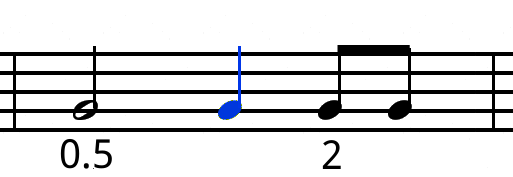
\includegraphics[width=0.4\textwidth]{fig/duration}
         \end{center}
         \caption{Duration from/to neighbor notes}
         \label{fig:duration}
      \end{figure}
   \item [Metric position:] The position of a note in a measure, measured by the beat unit defined by the time signature. For example, a $^4_4$ time signature will have a beat unit of a quarter note. So if the measure consists of four quarter notes, each of them will have metric position of 1, 2, 3 and 4. See figure \ref{fig:metrical}.

   \begin{figure}[tp]
      \begin{center}
         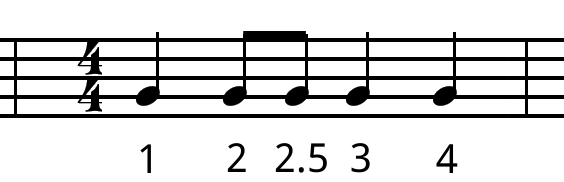
\includegraphics[width=0.4\textwidth]{fig/metrical}
      \end{center}
      \caption{Metric position}
      \label{fig:metrical}
   \end{figure}
      \end{description}

      %TODO: link to narmour group
   \begin{figure*}[tp]
      \begin{center}
         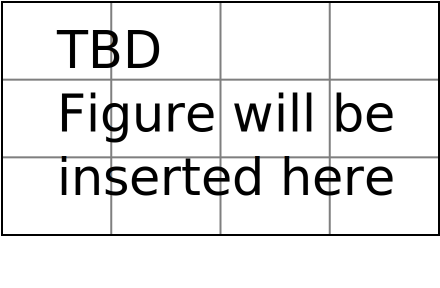
\includegraphics[width=0.8\textwidth]{fig/TBDFigure}
      \end{center}
      \caption{Example Score Features}
      \label{fig:expScoreFeat}
   \end{figure*}
      \subsection{Performance Features}
      Performance features includes:
      \begin{description}
         \item [Relative onset time bias:] 
            The onset time of a recording will not be exactly as the ones indicated on the score. Given a fixed tempo (beats/second), the score timing of each note can be calculated as tempo $\times$ (beats from the start of phrase)  . The relative onset time bias is the difference of onset timing between the performance and the score, divided by the total length of the phrase. Namely,
            $$ ROB = \frac{O_i^{perf} - O_i^{score}  }{length(phrase)}$$ Where $O_i^{perf}$ is the onset time of note $i$ in the performance, $O_i^{score}$ is the onset time of note $i$ in the score. 
         \item [Relative loudness:] The loudness of a note divided by the maximum loudness in the phrase. Measured by MIDI velocity level.
            $$ RL = \frac{L_i}{max(L_1, L_2, \dots, L_n)}$$

         \item [Relative duration:]
            The actual duration of note divided by the total length of the phrase.
            $$ RD = \frac{ D_i^{perf}}{length(phrase)}$$
      \end{description}

\begin{figure*}[tp]
   \begin{center}
      %TODO:Figure:Example JSON code
      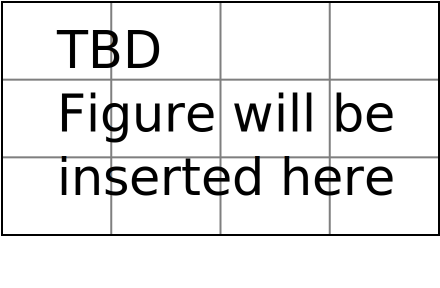
\includegraphics[width=\textwidth]{fig/TBDFigure}

   \end{center}
   \caption{Example Performance Features}
   \label{fig:expPerfFeat}
\end{figure*}
   % \section{Melodic Similarity and Sample Selection}
   % Once a score is given to the system for playing, all the samples in the database will be ranked by the melodic similarity with the given score. Here we use the melodic distance function provided by the MIDI Toolbox\cite{Eerola2004}, which is defined as follows: 
   % \begin{enumerate}
   %    \item Melodic contour is calculated by connecting each note's pitch, forming a piece-wise linear contour.
   %    \item Subtract the contour by it's mean to preserve only the relative part.
   %    \item If the two phrases has different length, re-sample both phrases with fixed intervals so both of the phrase will have contour vector of the same length.
   %    \item The L1 norm (a.k.a Taxicab distance) of these two contour vector is the similarity measure. 
   % \end{enumerate}
   % The reason I choose melodic contour is because it yields best results in finding melodic similarity, which is shown in \cite{Hoffmann-engl2005}.

      %TODO: not included features: e.g. notation
   \subsection{Normalizing Onset Timing}
\begin{figure}[tp]
   \begin{center}
      %TODO:Figure:Normalization Schemes
      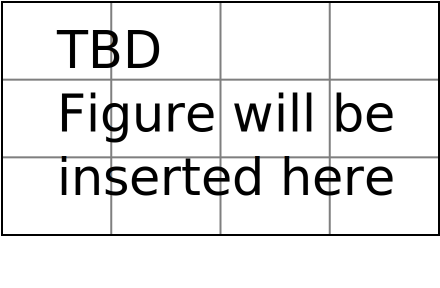
\includegraphics[width=\textwidth]{fig/TBDFigure}

   \end{center}
   \caption{Normalization Schemes}
   \label{fig:normalization}
\end{figure}
   The relative onset timing bias feature must be normalized to get meaningful result. For example, a phrase is played very fast by the performer, say, the played length is only 70\% of the notation. If the first note is aligned, the onset timing bias will grow linearly until the end of the phrase, the last note will have a onset timing bias of about 30\% of the phrase. But from the definition of this feature, the timing bias should be roughly less than half of  a note's length, and it's mean should be around zero. This 30\% value will introduce a relative large value in the training corpus, and thus there may be very large output value from the generation phase. If the model predict that a note should be played early or later for 30\% of the phrase length, the melody will be messed up. 

   There are four possible type of normalization: the first note can either be aligned at onset, or not aligned at all. The last note can be aligned at onset, or aligned at note off event.  The incentive for not aligning the first note is that the performer may intend to use an early start or delayed start as an expression, if the first note is aligned by it's onset, the first note in every phrase will have a onset timing bias feature of value zero. In other words, the early/delayed start expression is lost. %But each normalization method are equally reasonable theoretically, so we need to use empirical data to verify them. The experiment is explained in section \ref{TODO:experiment}. The experiment result showed that [TODO: result]
   But experiments shows that none of these methods can fit all training samples. One may get good result by using one method on part of the corpus, but may result in large bias when applying it to the rest of the corpus. Since none of the methods can fit all, we take a different approach: let the program find the best fitting ratio for normalization. To achieve this goal, we first have to define how "fit" two phrases are, or how to define the distance between phrase. If the onset time of all the notes in a phrase are concatenated into a vector, the $l^2$-norm of the tow vectors can be treated as the distance. Note that the two vectors must have the same size, because the recordings are required to match note-to-note with the score. So the problem becomes how to find a optimal scaling ratio such that the scaled recording has the minimum distance from the score. The Brent's method\cite{TODO:brent1973} is used to find the optimal ratio. To speed up the optimization and prevent extreme values, we imposed a range of $[initial_guess \times 0.5 , initial_guess \times 2]$ to the optimizer. The $initial_guess$ is used as a rough estimate of the ratio, calculated by aligning the first and last onset of the phrase. Than we assume the actual ratio will not be smaller than half of $initial_guess$ and not larger than twice of $initial_guess$. The two numbers 0.5 and 2 are arbitrary chosen, but most of the empirical data suggest is valid most of the time. 
   \framebox{TODO: conclusion}


   %TODO:Automatic onset timing normalization
   %TODO:Define the distance
   %TODO:SciPy optimization method


      %TODO: 4 onset diffs
